%%%%%%%%%%%%%%%%%%%%%%%%%%%%%%%%%%%%%%%%%%%%%%%%%%%%
% コンパイル:
%   xelatex main.tex && xelatex main.tex
%%%%%%%%%%%%%%%%%%%%%%%%%%%%%%%%%%%%%%%%%%%%%%%%%%%%
\documentclass[10pt,twocolumn]{AROB}
\usepackage{amssymb}
\usepackage{amsmath}
\usepackage{multirow}
\usepackage{url}
\usepackage{xcolor}
\usepackage{graphicx}
\usepackage{booktabs}
\newtheorem{definition}{定義}
\newtheorem{lemma}{補題}
\usepackage{algorithm}
\usepackage{algpseudocode}
\usepackage{xeCJK}
\setCJKmainfont[AutoFakeBold=2.5]{Hiragino Mincho ProN}
\setCJKsansfont{Hiragino Sans}
\setCJKmonofont{Hiragino Sans}

\title{Streaming Apriori-Window: Mining Dense Patterns\\
       from Streaming Data for Autonomous Agent Monitoring}

\author{Kanata Takayasu${}^{1\dagger}$, Taihei Takahashi${}^{1}$,
        Satoshi Suga${}^{2}$, and Satoshi Kurihara${}^{1}$}
% The dagger symbol indicates the presenter.
\speaker{Kanata Takayasu}

\affils{${}^{1}$Keio University, Yokohama, Japan\\
${}^{2}$Kansai University, Osaka, Japan\\
}

\abstract{%
自律AIシステムおよびロボットエージェントは、行動パターンを内包したセンサイベントストリームを生成する。
これらのパターンが\textit{いつ}密集して共起するかを検出するには、出力レイテンシを制御可能な
ストリーミング対応の区間マイニングフレームワークが必要である。
本稿では、スキャン頻度 $\Delta$ をパラメータとする Streaming Apriori-Window を提案する。
提案手法は、固定幅スライディングウィンドウ内でアイテムセット頻度が閾値を満たす
すべての時間区間を特定する。
単調スキャン性質から確定出力保証が得られる。
Scan Stride Skipping と Apriori Interval Pruning の2つの高速化技術により実用的な処理速度を実現する。
合成データおよび実データを用いた4つの実験で評価する：
パラメータ感度分析（EX-1）、スケーラビリティ実験（EX-2）、
両高速化技術が独立に寄与することを確認するアブレーション実験（EX-3）、
および解釈可能かつドメイン整合的な密集区間を出力する
CASASスマートホームセンサストリームを用いた実データ評価（EX-4）。\par
これらの実験から、提案手法が実用的な処理速度でストリームデータからの密集パターンを正確に抽出でき、
自律エージェント監視への適用可能性を持つことが示された。%
}

\keywords{%
Data Streaming Mining, Dense Pattern Mining, Sensor Data Analysis,
Behavior Analysis, Intelligent Monitoring%
}

\begin{document}

\maketitle

%-----------------------------------------------------------------------

%%%%%%%%%%%%%%%%%%%%%%%%%%%%%%%%%%%%%%%%%%%%%%%%%%%%
\section{はじめに}

自律AIシステムおよびロボットエージェントは、行動パターンを内包したセンサイベントストリームを生成する。
これらのパターンが「いつ」密集して共起するかを理解すること、単にグローバルに頻出するかどうかではなく、
は、知的環境におけるリアルタイム監視・異常検知・適応制御に不可欠である。
マルチエージェントシステムやセンサ搭載ロボットプラットフォームでは、特定のイベント集合が特定の時間区間に
密集していることを検出することで、協調行動・日常ルーティン・迅速な対応を要する異常の出現を
明らかにすることができる。
また、この手法は小売や疫学などの幅広い分野へも適用可能である。

本稿では、スキャン頻度 $\Delta$ をパラメータとする密集区間マイニングアルゴリズム
\textit{Streaming Apriori-Window} を提案する。
アルゴリズムは、固定幅スライディングウィンドウ内でのアイテムセット出現頻度が閾値を満たす
すべての時間区間を特定する。
2つの高速化技術、Scan Stride Skipping と Apriori Interval Pruning を組み込み、
実用的な処理速度を実現する。
著者らは予備的研究~\cite{takayasu2025arxiv}においてApriori-Windowを提案した。
本稿では、これをストリーミングフレームワークへ拡張し、形式的な出力保証、高速化技術の証明、
および包括的な実験評価を加える。

本稿の主な貢献は以下の通りである：
\begin{itemize}
  \item 出力レイテンシと処理コストのトレードオフを制御する明示的なスキャン頻度パラメータ $\Delta$ を持つ
        ストリーミング密集区間マイニング問題を形式化する。
  \item 確定出力保証を示す：現在のスキャン位置より前に終端する区間は、将来のイベントによって変化しない。
  \item 合成データおよびCASASスマートホームセンサデータを用いた4つの実験により、実用的な処理速度と
        解釈可能な出力を実証する。
\end{itemize}


%%%%%%%%%%%%%%%%%%%%%%%%%%%%%%%%%%%%%%%%%%%%%%%%%%%%
\section{関連研究}

\subsection{頻出アイテムセットマイニング}

Apriori~\cite{agrawal1994fast} と FP-Growth~\cite{han2000mining} は頻出アイテムセットマイニング（FIM）の
基盤となる手法である。
ECLAT~\cite{zaki1997new} は垂直データ形式を用いた代替手法を提供する。
FIM の包括的な調査は~\cite{fournier2017survey,luna2019fim,fournierviger2022survey} に詳しい。
周期的頻出パターンマイニング PFPM~\cite{tanbeer2009pfpm} や，
複数の最小サポートを導入して希少アイテム問題~\cite{liu1999multiple} に対処する研究も存在するが，
いずれもグローバルな評価に依存する点は変わらない。
これらの手法はいずれもデータセット全体でサポートを評価するため、特定の時間区間でのみ高頻度で出現する
アイテムセットを検出できない。

\subsection{密集区間マイニング}

パターンとその密集区間を同時に出力する手法は2種類に大別される。
\textit{発生ギャップ型}手法には、LPFIM~\cite{yin2014lpfim}、LPPM~\cite{saleh2011lppm}、
RPM~\cite{kiran2017rpm} がある。
LPFIM は出現ギャップが閾値に達したとき区間を分割し、LPPM はノイズロバストな検出のために
累積スピルオーバーを導入し、RPM は最大周期内のギャップで連続する出現をグループ化する。
これらの手法はギャップ制約や周期閾値を通じて密度を間接的に推定するため、パラメータ調整が困難であり、
直接的なスライディングウィンドウ頻度に対して結果が近似的となる。
\textit{直接型}手法としては、固定時間粒度でパターンをマイニングするため任意幅の区間を特定できない
GLFMiner~\cite{fournierviger2021glf} と、アイテムセットごとに最適な単一区間のみを返す
SIM~\cite{kiran2015sim} がある。
これらの手法はいずれもストリーミングをサポートせず、スキャン頻度を制御する機構を持たない。

\subsection{ストリームマイニング}

スライディングウィンドウを用いたストリームマイニングはインクリメンタルFIM として研究されており
~\cite{lee2001sliding,leung2006dstree}、ウィンドウがサポート計算の時間的スコープを制限する。
しかしこれらの手法はウィンドウ内のグローバルサポートを報告するものであり、
すべての密集部分区間を列挙しない。
バースト検出~\cite{kleinberg2003bursty,yang2021burstsketch} はストリーム中の
頻度スパイクを検出するが、アイテムセット共起の密集区間は列挙しない。

\subsection{本研究の立ち位置}

密集パターンの本質は、あるアイテムセットが特定の連続区間内でのみ局所的に高頻度で出現する点にある。
本研究では、スライディングウィンドウを用いてウィンドウ内の出現頻度を直接評価することで、
発生ギャップ制約に依存せずに局所密度を定量化する。
これによりパラメータ感度問題を原理的に回避できる。

既存の手法群を整理すると、(1) パターンのみを出力するFIM系手法、(2) パターンと区間を同時に出力するが
ギャップ制約経由で密度を間接推定するLPFIM/LPPM/RPM、(3) 直接的な局所頻度を評価するが
区間の粒度や個数に制限があるGLFMiner/SIM、(4) ストリームマイニングではあるが密集部分区間を
列挙しないインクリメンタルFIM、のいずれも「スライディングウィンドウによる直接的な局所頻度評価」と
「アイテムセットの反単調性を組み合わせた密集区間の網羅的列挙」を
ストリーミング環境で実現するものではない。
本稿はこの方向性をストリーミング対応アルゴリズムとして定式化・実装する試みである。


%%%%%%%%%%%%%%%%%%%%%%%%%%%%%%%%%%%%%%%%%%%%%%%%%%%%
\section{問題定式化}

\subsection{ストリーミング型イベントストリーム}

$\mathcal{I}$ をアイテムの有限集合とする。
\textbf{イベントストリーム}は、$I_t \subseteq \mathcal{I}$ を満たすイベントの列
$I_0, I_1, I_2, \ldots$ であり、各イベントには離散タイムスタンプ $t \in \mathbb{Z}_{\geq 0}$ が付与される。
センサ観測やエージェントログのように、イベントは時間の経過とともに逐次生成され、
終端が事前に定まらない点がストリームの本質的な特徴である。

\subsection{密集区間}

ウィンドウ幅 $W \in \mathbb{Z}_{>0}$ および閾値 $\theta \in \mathbb{Z}_{>0}$ を与える。

\begin{definition}[区間サポート]
パターン $X \subseteq \mathcal{I}$ の発生列を
$\mathit{occ}(X) = \{t : X \subseteq I_t\}$ とする。
ウィンドウ左端 $l$ における\textbf{区間サポート}を
\[
  \mathrm{sup}(X, l, W) = |\{t \in \mathit{occ}(X) : l \leq t \leq l + W\}|
\]
と定義する。窓 $[l,\, l{+}W]$ は $W{+}1$ 個の離散時刻を含む。
\end{definition}

\begin{definition}[密集開始点集合と密集区間]
サポート閾値 $\theta$ に対し、
\[
  \mathcal{T}_\theta(X) = \{l \in \mathbb{Z}_{\geq 0} : \mathrm{sup}(X, l, W) \geq \theta\}
\]
を $X$ の\textbf{密集開始点集合}とする。
$[a,\, b] \subseteq \mathcal{T}_\theta(X)$ の最大連続成分に対し、
$[a,\, b{+}W]$ を $X$ の\textbf{密集区間}と呼ぶ。
\end{definition}

\subsection{ストリーミング密集区間マイニング問題}

センサや自律エージェントが生成するイベントストリームでは、
イベントが継続的に到着し続ける。
システムは $\Delta$ 秒ごとに定期的にスキャンをトリガーし、
そのスキャン時点 $s$ までに受信済みのイベント列に対して密集区間を計算する。
スキャン時刻 $s = 0, \Delta, 2\Delta, \ldots$ において、
右端が $l_e + W \leq s$ を満たすすべての密集区間 $(X, [l_s, l_e])$ を重複なく列挙することが目標である。

パラメータ $\Delta$ はレイテンシと計算コストのトレードオフを制御する。
$\Delta$ を小さく設定するほどスキャン頻度が上がり、
低いレイテンシでリアルタイムに密集区間を検出できる。


%%%%%%%%%%%%%%%%%%%%%%%%%%%%%%%%%%%%%%%%%%%%%%%%%%%%
\section{アルゴリズム}

\subsection{手法概要}

Apriori-Window は、Apriori の反単調性~\cite{agrawal1994fast}を
スライディングウィンドウ局所頻度評価に適用した厳密列挙アルゴリズムである。
入力はイベントストリーム、ウィンドウ幅 $W$、閾値 $\theta$、
およびスキャン頻度 $\Delta$ であり、
出力は全密集パターン $X$ とその密集区間集合 $\mathrm{DI}(X)$ の列挙である。

アルゴリズムはアイテムセットサイズ $k = 1$ から始まり、
サイズ $k$ の密集パターン集合 $L_k$ からサイズ $k{+}1$ の候補を生成し、
各候補の密集区間を計算することを繰り返す。
各アイテムセット $X$ の密集区間計算では、
ウィンドウ $[l, l{+}W]$ 内の $X$ の出現数をカウントしながら左から右へスライドさせる。
このスライド幅を動的に調整する Scan Stride Skipping により、
不要なスキャンを省いて計算コストを削減する。
さらに Apriori の反単調性を用いた候補区間の枝刈り、
Apriori Interval Pruning により探索空間を絞り込む。

スキャンは $\Delta$ 秒ごとにトリガーされ、
直前の走査終端位置を引き継いで新着イベントを対象に走査を継続する。
$\Delta$ を小さくするほどリアルタイム性が向上し、
大きくするほど Scan Stride Skipping の恩恵によりスキャン回数が減り計算コストが下がる。

アルゴリズム~\ref{alg:aw} に全体手順を示す。
$\mathrm{Scan}$ は Scan Stride Skipping を適用した単調スキャンであり、
候補スキャン範囲 $R_X$ は Apriori Interval Pruning で計算する。

\begin{algorithm}[t]
\caption{Apriori-Window（単一スキャン）}\label{alg:aw}
\begin{algorithmic}[1]
\Require $\mathit{occ}$：アイテム$\to$発生位置列マップ；$W$；$\theta$
\Ensure $F$：パターン$\to$密集区間集合マップ
\State $F \leftarrow \emptyset$；$L_1 \leftarrow \emptyset$
\For{$x \in \mathrm{sorted}(\mathrm{keys}(\mathit{occ}))$}
  \State $\mathrm{DI}(x) \leftarrow \mathrm{Scan}(\mathit{occ}(x),\, W,\, \theta,\, \text{全範囲})$
  \If{$\mathrm{DI}(x) \neq \emptyset$}
    \State $F[\{x\}] \leftarrow \mathrm{DI}(x)$；$L_1 \leftarrow L_1 \cup \{\{x\}\}$
  \EndIf
\EndFor
\State $k \leftarrow 2$；$L_p \leftarrow L_1$
\While{$L_p \neq \emptyset$}
  \State $C_k \leftarrow \mathrm{AprioriJoin}(L_p)$
  \State $L_k \leftarrow \emptyset$
  \For{$X \in C_k$}
    \State $\mathit{occ}(X) \leftarrow \bigcap_{x \in X} \mathit{occ}(x)$
    \If{$\mathit{occ}(X) = \emptyset$} \textbf{continue} \EndIf
    \State $R_X \leftarrow \mathrm{cand}(X)$
    \If{$R_X = \emptyset$} \textbf{continue} \EndIf
    \State $\mathrm{DI}(X) \leftarrow \mathrm{Scan}(\mathit{occ}(X),\, W,\, \theta,\, R_X)$
    \If{$\mathrm{DI}(X) \neq \emptyset$}
      \State $F[X] \leftarrow \mathrm{DI}(X)$；$L_k \leftarrow L_k \cup \{X\}$
    \EndIf
  \EndFor
  \State $L_p \leftarrow L_k$；$k \leftarrow k + 1$
\EndWhile
\State \Return $F$
\end{algorithmic}
\end{algorithm}

\subsection{Scan Stride Skipping}

$l$ を毎ステップ1ずつインクリメントするナイーブな方法は非効率である。
そのため、スキャンせずとも確実に密集・非密集が判定できる区間はスキャンをスキップする。

固定アイテムセット $X$ に対し、$\mathit{occ}(X)$ を $X$ が出現するタイムスタンプのソート済みリストとする。
ウィンドウ $[l, l{+}W]$ 内のアイテムセット $X$ の出現数を $c$ とする。
$c$ と $\theta$ の大小に応じた2分岐のストライドにより $l$ を更新することで、確実に密集・非密集が判定できる区間はスキャンをスキップする。（図~\ref{fig:scan_stride}）。

\textbf{密集フェーズ}（$c \geq \theta$）：
$i_{\mathrm{start}}$ をウィンドウ内の最初の出現インデックスとする。
ウィンドウを右にスライドさせて、余剰 $c - \theta$ の分がウィンドウ外に出たとしても、閾値以上であることは保証される。
したがって、区間 $[l,\, \mathit{occ}(X)[i_{\mathrm{start}} + c - \theta] + W]$ を密集区間として出力したうえで、
以下のように$l$ を更新し、次のスキャンを開始する：
\begin{equation}\label{eq:stride_dense}
  l \leftarrow \mathit{occ}(X)[i_{\mathrm{start}} + c - \theta] + 1.
\end{equation}

\textbf{非密集フェーズ}（$c < \theta$）：
$i_{\mathrm{end}}$ をウィンドウ直後の最初の出現インデックスとする。
ウィンドウ内の出現数は $c < \theta$ であり、次に密集となりうる最小の左端は
不足分 $\theta - c$ 個の出現を新たに取り込む位置である。
したがって、以下のように $l$ をジャンプさせ、次のスキャンを開始する：
\begin{equation}\label{eq:stride_sparse}
  l \leftarrow \mathit{occ}(X)[i_{\mathrm{end}} + (\theta - c) - 1] - W.
\end{equation}

両フェーズの正当性は付録~B（補題~\ref{lem:stride_dense}，補題~\ref{lem:stride_sparse}）に示す。

\begin{figure}[t]
\centering
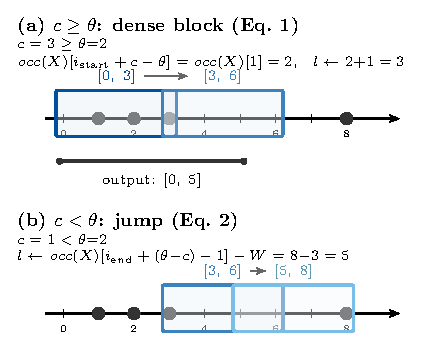
\includegraphics[width=\columnwidth]{fig/scan_stride.pdf}
\caption{Scan Stride Skipping の動作（式~\eqref{eq:stride_dense}，\eqref{eq:stride_sparse}）。}
\label{fig:scan_stride}
\end{figure}

\subsection{Apriori Interval Pruning}

古典的 Apriori~\cite{agrawal1994fast} の反単調性（anti-monotonicity）は
「頻出アイテムセットの任意の部分集合も頻出である」という性質であり、
対偶をとれば「ある部分集合が非頻出ならそのスーパーセットも必ず非頻出」となる。
本手法ではこれを\textit{区間単位}で適用する。
$Y \subseteq X$ ならば $X$ が時刻 $t$ に出現するときは常に $Y$ も出現するから、
任意のウィンドウ $[l, l+W]$ に対して
\[
  \mathrm{sup}(X, l, W) \leq \mathrm{sup}(Y, l, W)
\]
が成り立つ（補題~\ref{lem:apriori}、付録~C）。
すなわち $[l, l+W]$ が $Y$ の密集区間でなければ $X$ の密集区間にもなりえない。
よってサイズ $k$ の候補 $X$ が密集しうる左端 $l$ は、
全 $(k{-}1)$ 部分集合が密集する $l$ 値集合の共通部分に限定される：
\begin{equation}\label{eq:cand}
  R_X = \bigcap_{Y \subsetneq X,\, |Y|=k-1} \mathcal{T}_\theta(Y),
\end{equation}
ここで $\mathcal{T}_\theta(Y)$ は $Y$ が密集する左端の集合である。
$R_X$ に含まれない $l$ は安全にスキップでき、スキャン範囲を大幅に削減できる。


\subsection{$\Delta$-ステップストリーミング}

対象デプロイメントでは、イベントがセンサストリームまたは自律エージェントログから継続的に到着し
データベースに追記される。
システムは $\Delta$ 秒ごとにスキャンをトリガーする。

各スキャンステップは以下のように進行する：

\begin{enumerate}
  \item $\Delta$ 秒が経過したとき（現在位置 $s$）、バッファ $[s - W + 1,\; s + \Delta)$ を取得し、
        境界損失を防ぐため直前ステップから最新 $W{-}1$ 件のイベントを保持する。
  \item Scan Stride Skipping および Apriori Interval Pruning を適用した単調スキャンを
        このバッファに対して実行する。
  \item まだ出力していない $l_e + W \leq s$ を満たすすべての区間 $(X, [l_s, l_e])$ を出力する：
        これらは\textbf{確定}しており、将来のイベントによって変化しない。
  \item 次の $\Delta$ 件のイベント蓄積まで待機し、繰り返す。
\end{enumerate}


%%%%%%%%%%%%%%%%%%%%%%%%%%%%%%%%%%%%%%%%%%%%%%%%%%%%
\section{実験}\label{sec:experiments}

全実験は Apple M3 Pro（18\,GB RAM）上で Rust~1.82 リリースビルドを用いて実施した。
到着レイテンシとは独立に\textit{純計算時間}を計測するため、
データセット全体をプリロードし $\Delta$ 件ずつ供給して
各スキャン完了直後に次のスキャンをトリガーする。

%-----------------------------------------------------------------------
\subsection{EX-1: スキャン頻度パラメータ感度分析}\label{sec:ex1}
%-----------------------------------------------------------------------

スキャン頻度パラメータ $\Delta$ が総処理時間に与える影響を定量化し、
出力レイテンシと計算コストのトレードオフを明らかにする。
合成ストリーム（$T = 10{,}000$、$|\mathcal{I}| = 20$、$W = 24$、$\theta = 10$、
生成方法は付録Aを参照）に対して $\Delta \in \{1, 10, 100, 1{,}000, 10{,}000\}$ を変化させた。

\begin{figure}[t]
\centering
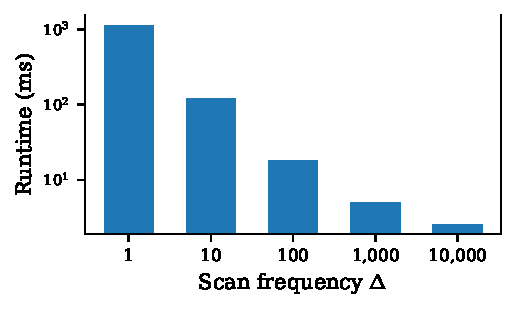
\includegraphics[width=\columnwidth]{fig/ex1_h_vs_time.pdf}
\caption{スキャン頻度 $\Delta$ vs. 処理時間（対数軸）.}
\label{fig:ex1}
\end{figure}

図\ref{fig:ex1}に示す通り、$\Delta$ を10倍にするごとに処理時間は概ね10分の1となり、
スキャン回数の削減が直接的に処理コストを削減することが確認された。

%-----------------------------------------------------------------------
\subsection{EX-2: スケーラビリティ}\label{sec:ex2}
%-----------------------------------------------------------------------

ストリーム長 $T$ およびアイテム数 $|\mathcal{I}|$ を独立に変化させ、
処理時間とピークメモリ使用量がどのようにスケールするかを検証する。
$\Delta = T$（バッチ処理）として実行し純計算時間のみを計測した。
合成データ（$\theta = 10$、$W = 120$）に対して $T$・$|\mathcal{I}|$ を独立に変化させた。
基準設定は $T = 10^{5}$、$|\mathcal{I}| = 24$ とし、各軸の変化時は他のパラメータを固定した。

\begin{figure}[t]
\centering
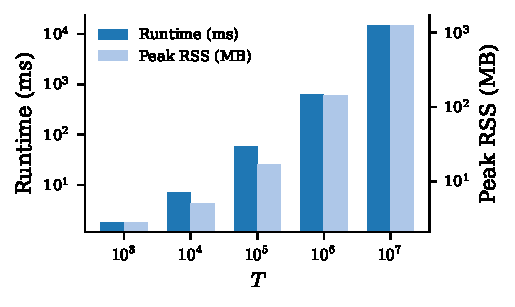
\includegraphics[width=\columnwidth]{fig/ex2_scalability_T.pdf}
\caption{スケーラビリティ vs. $T$：Runtime および Peak RSS.}
\label{fig:ex2t}
\end{figure}

\begin{figure}[t]
\centering
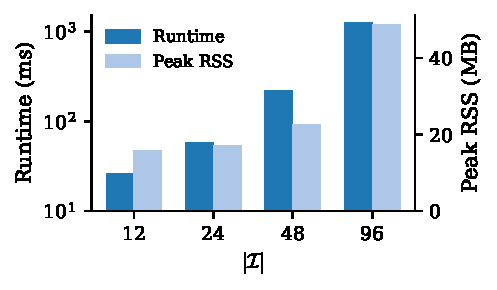
\includegraphics[width=\columnwidth]{fig/ex2_scalability_N.pdf}
\caption{スケーラビリティ vs. $|\mathcal{I}|$：Runtime および Peak RSS.}
\label{fig:ex2n}
\end{figure}

図\ref{fig:ex2t}に示す通り、処理時間は $T$ に対してほぼ線形にスケールし、
$T = 10^{6}$ で 636\,ms、$T = 10^{7}$ で 15{,}108\,ms となった。
図\ref{fig:ex2n}より、$|\mathcal{I}|$ に対しては超線形スケールを示す（$|\mathcal{I}|=96$ で 1{,}272\,ms）が、
これは $|\mathcal{I}|$ 増加により Apriori の高次候補が組み合わせ的に増加するためである。
Peak RSS は $T$ に対してほぼ線形に増加し、$|\mathcal{I}|$ への依存は小さい。

%-----------------------------------------------------------------------
\subsection{EX-3: アブレーション実験}\label{sec:ex3}
%-----------------------------------------------------------------------

Scan Stride Skipping と Apriori Interval Pruning のそれぞれの独立した寄与を定量化し、
両技術を組み合わせることの効果を確認する。
$\Delta = T$（バッチ処理）として実行し純計算時間のみを計測した。
合成データ（$T = 100{,}000$、$|\mathcal{I}| = 48$、$W = 120$、$\theta = 50$、
エポック重複幅 100）に対して下記の4構成の処理時間を計測した。


\begin{figure}[t]
\centering
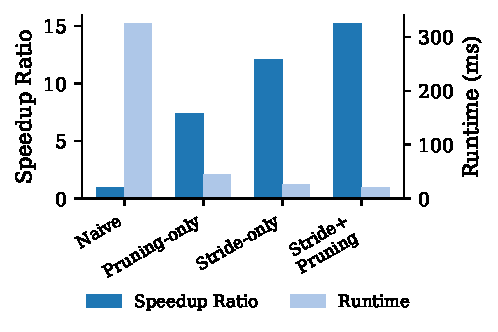
\includegraphics[width=\columnwidth]{fig/ex3_speedup.pdf}
\caption{アブレーション：Naive を基準とした高速化倍率.}
\label{fig:ex3}
\end{figure}

図\ref{fig:ex3}に処理時間および Naive を 1.00 とした高速化倍率を示す。
Full（21.4\,ms）はすべての個別構成を上回る。
Scan Stride Skipping が主要な寄与因子であり、
Naive 比 12.1$\times$ の高速化をもたらす。
Apriori Interval Pruning は単独では 7.4$\times$ の高速化をもたらし、
Stride Skipping と組み合わせることで 15.2$\times$ の高速化を実現する。
2つの技術は独立かつ相補的に寄与することが確認された。

%-----------------------------------------------------------------------
\subsection{EX-4: CASAS センサデータへの適用}\label{sec:ex4}
%-----------------------------------------------------------------------

実センサストリームに提案手法を適用し、
検出された密集区間が解釈可能な行動ルーティンに対応することを確認する。
CASAS スマートホームデータセット~\cite{casas2013} の2系列（hh113・mv001）を使用した。
CASAS は住居内のモーション・接触センサの発火ストリームを記録したものであり、
自律エージェントの行動ログと構造的に類似する。

センサ発火を15分ごとの時間スロットに集約して前処理した（スロット幅 $=$ 15分）。
ウィンドウサイズを $W = 24$スロット（$= 6$時間）に設定し、
1日の特定の時間帯（朝・夕・夜）における行動ルーティンを捕捉できるよう設計した。
スキャン頻度は $\Delta = W = 24$ とした。
各データセットの概要と検出パターン数を表\ref{tab:casas_stats}に示す。

\begin{table}[t]
\caption{CASAS データセット統計.}
\label{tab:casas_stats}
\begin{center}
\begin{tabular}{ccccc}
\hline
データセット & $T$ & $|\mathcal{I}|$ & $\theta$ & パターン数 \\\hline
hh113 & 48{,}901 & 7 & 14 & 26 \\
mv001 & 139{,}033 & 7 & 18 & 34 \\\hline
\end{tabular}
\end{center}
\end{table}

代表的な検出パターンを表\ref{tab:casas_hh113}・表\ref{tab:casas_mv001}に示す。
hh113 では食事関連パターン（DiningRoom+Kitchen：45区間）が卓越し、
キッチン・ダイニングを中心とした日常ルーティンが6時間ウィンドウ内で
繰り返し形成されていることを示す。
mv001 では就寝前の遷移パターン（Bedroom+LivingRoom：113区間）が最頻であり、
リビング滞在 $\to$ 調理 $\to$ 就寝という行動シーケンスが日課として定着していることが示唆される。
いずれのデータセットでも $k \geq 3$ の多アイテムパターンが自動列挙され、
二者間共起では捉えられない複合的な行動遷移が可視化された。

\begin{table}[t]
\caption{hh113における代表的な検出パターン}
\label{tab:casas_hh113}
\begin{center}
\footnotesize
\begin{tabular}{p{3.5cm}cp{2.0cm}}
\hline
センサ組合せ & 区間数 & 推定行動 \\\hline
DiningRoom + Kitchen              & 45 & 食事準備・食事行動 \\
Bathroom + Bedroom                &  8 & 起床・就寝ルーティン \\
DiningRoom + Kitchen + OutsideDoor &  7 & 外出前後の食事行動 \\\hline
\end{tabular}
\end{center}
\end{table}

\begin{table}[t]
\caption{mv001における代表的な検出パターン}
\label{tab:casas_mv001}
\begin{center}
\footnotesize
\begin{tabular}{p{3.5cm}cp{2.0cm}}
\hline
センサ組合せ & 区間数 & 推定行動 \\\hline
Bedroom + LivingRoom          & 113 & 就寝前リビング→寝室 \\
Kitchen + LivingRoom          &  66 & 調理後リビング滞在 \\
Bedroom + Kitchen             &  44 & 就寝前・起床直後 \\
Bedroom + Kitchen + LivingRoom &  44 & 夕方〜就寝前連鎖 \\\hline
\end{tabular}
\end{center}
\end{table}


%%%%%%%%%%%%%%%%%%%%%%%%%%%%%%%%%%%%%%%%%%%%%%%%%%%%
\section{おわりに}

本稿では、明示的なスキャン頻度パラメータ $\Delta$ を持つイベントストリーム向け密集区間マイニングアルゴリズム
Streaming Apriori-Window を提案した。
確定出力保証は単調スライディングウィンドウの性質から導かれ、出力された区間が将来のイベントによって
無効化されないことを保証する。
2つの高速化技術、Scan Stride Skipping と Apriori Interval Pruning により処理コストを大幅に削減し、
$\Delta = W$ でレイテンシと処理速度の良好なトレードオフを実現する。
CASAS スマートホームセンサデータを用いた実験により、アルゴリズムが解釈可能かつドメイン整合的な出力を
生成することが実証され、自律エージェント監視への実用性が確認された。

今後の課題として、物理ロボットシステムから収集した行動ログへのフレームワークの適用、
多次元イベント空間への拡張、ストリーム特性に基づく適応的スキャン頻度機構の研究に取り組む予定である。


%-----------------------------------------------------------------------

\section*{Acknowledgment}
This work is supported by the Honda Bridge Project.
Part of the text in this paper was generated with assistance from Anthropic's large language model Claude~\cite{claude2025}.

%-----------------------------------------------------------------------

\begin{thebibliography}{99}

\bibitem{takayasu2025arxiv}
K. Takayasu {\it et al.},
``Apriori-Window: Exact enumeration of dense itemset intervals over sliding windows,''
{\it arXiv preprint arXiv:2604.24122}, 2025.

\bibitem{agrawal1994fast}
R. Agrawal and R. Srikant,
``Fast algorithms for mining association rules,''
in \textit{Proceedings of the 20th International Conference on Very Large Data Bases (VLDB'94)},
pp.~487--499, 1994.

\bibitem{zaki1997new}
M. J. Zaki, S. Parthasarathy, M. Ogihara, and W. Li,
``New algorithms for fast discovery of association rules,''
in \textit{Proceedings of the 3rd ACM SIGKDD International Conference on Knowledge Discovery and Data Mining (KDD'97)},
pp.~283--296, 1997.

\bibitem{han2000mining}
J. Han, J. Pei, and Y. Yin,
``Mining frequent patterns without candidate generation,''
\textit{ACM SIGMOD Record}, vol.~29, no.~2, pp.~1--12, 2000.
DOI: \url{https://doi.org/10.1145/335191.335372}.

\bibitem{fournier2017survey}
P. Fournier-Viger, J. C.-W. Lin, B. Vo, T. T. Chi, J. Zhang, and H. B. Le,
``A survey of itemset mining,''
{\it WIREs Data Mining Knowl. Discov.}, vol.~7, no.~4, e1207, 2017.
DOI: \url{https://doi.org/10.1002/widm.1207}.

\bibitem{yin2014lpfim}
K.-C. Yin, Y.-L. Hsieh, D.-L. Yang, and M.-C. Hung,
``Association rule mining considering local frequent patterns with temporal intervals,''
{\it Applied Mathematics \& Information Sciences}, vol.~8, no.~4,
pp.~1879--1890, 2014.
DOI: \url{https://doi.org/10.12785/amis/080446}.

\bibitem{saleh2011lppm}
B. Saleh and F. Masseglia,
``Discovering frequent behaviors: Time is an essential element of the context,''
{\it Knowledge and Information Systems}, vol.~28, no.~2, pp.~311--331, 2011.
DOI: \url{https://doi.org/10.1007/s10115-010-0361-5}.

\bibitem{kiran2017rpm}
R. U. Kiran, J. Venkatesh, M. Toyoda, M. Kitsuregawa, and P. K. Reddy,
``Discovering partial periodic-frequent patterns in a transactional database,''
{\it Journal of Systems and Software}, vol.~125, pp.~170--182, 2017.
DOI: \url{https://doi.org/10.1016/j.jss.2016.11.035}.

\bibitem{fournierviger2021glf}
P. Fournier-Viger, P. Yang, R. U. Kiran, S. Ventura, and J. M. Luna,
``Mining local periodic patterns in a discrete sequence,''
{\it Information Sciences}, vol.~544, pp.~519--548, 2021.
DOI: \url{https://doi.org/10.1016/j.ins.2020.09.044}.

\bibitem{kiran2015sim}
R. U. Kiran, H. Shang, M. Toyoda, and M. Kitsuregawa,
``Discovering recurring patterns in time series,''
in \textit{Proceedings of the 18th International Conference on Extending Database Technology (EDBT 2015)},
pp.~97--108, 2015.

\bibitem{lee2001sliding}
C.-H. Lee, C.-R. Lin, and M.-S. Chen,
``Sliding-window filtering: An efficient algorithm for incremental mining,''
in \textit{Proceedings of the 10th ACM Conference on Information and Knowledge Management (CIKM 2001)},
pp.~263--270, 2001. DOI: \url{https://doi.org/10.1145/502585.502630}.

\bibitem{leung2006dstree}
C. K.-S. Leung and Q. I. Khan,
``DSTree: A tree structure for the mining of frequent sets from data streams,''
in \textit{Proceedings of the 6th IEEE International Conference on Data Mining (ICDM 2006)},
pp.~928--932, 2006. DOI: \url{https://doi.org/10.1109/ICDM.2006.62}.

\bibitem{luna2019fim}
J. M. Luna, P. Fournier-Viger, and S. Ventura,
``Frequent itemset mining: A 25 years review,''
{\it WIREs Data Mining and Knowledge Discovery}, vol.~9, no.~6, e1329, 2019.
DOI: \url{https://doi.org/10.1002/widm.1329}.

\bibitem{fournierviger2022survey}
P. Fournier-Viger, W. Gan, Y. Wu, M. Nouioua, W. Song, T. Truong, and H. D. Van,
``Pattern mining: Current challenges and opportunities,''
in \textit{Database Systems for Advanced Applications: DASFAA 2022 International Workshops},
Lecture Notes in Computer Science, vol.~13248, pp.~34--49, Springer, 2022.
DOI: \url{https://doi.org/10.1007/978-3-031-11217-1_3}.

\bibitem{liu1999multiple}
B. Liu, W. Hsu, and Y. Ma,
``Mining association rules with multiple minimum supports,''
in \textit{Proceedings of the 5th ACM SIGKDD International Conference on Knowledge Discovery and Data Mining (KDD'99)},
pp.~337--341, 1999. DOI: \url{https://doi.org/10.1145/312129.312274}.

\bibitem{tanbeer2009pfpm}
S. K. Tanbeer, C. F. Ahmed, B.-S. Jeong, and Y.-K. Lee,
``Discovering periodic-frequent patterns in transactional databases,''
in \textit{Advances in Knowledge Discovery and Data Mining: 13th Pacific-Asia Conference (PAKDD 2009)},
Lecture Notes in Computer Science, vol.~5476, pp.~242--253, Springer, 2009.
DOI: \url{https://doi.org/10.1007/978-3-642-01307-2_24}.

\bibitem{kleinberg2003bursty}
J. Kleinberg,
``Bursty and hierarchical structure in streams,''
{\it Data Mining Knowl. Discov.}, vol.~7, no.~4, pp.~373--397, 2003.
DOI: \url{https://doi.org/10.1023/A:1024940629314}.

\bibitem{yang2021burstsketch}
Z. Zhong, S. Yan, Z. Li, D. Tan, T. Yang, and B. Cui,
``BurstSketch: Finding bursts in data streams,''
in \textit{Proceedings of the 2021 International Conference on Management of Data (SIGMOD'21)},
pp.~2375--2383, 2021. DOI: \url{https://doi.org/10.1145/3448016.3452775}.

\bibitem{casas2013}
D. J. Cook, A. S. Crandall, B. L. Thomas, and N. C. Krishnan,
``CASAS: A smart home in a box,''
{\it Computer}, vol.~46, no.~7, pp.~62--69, 2013.
DOI: \url{https://doi.org/10.1109/MC.2012.328}.

\bibitem{claude2025}
Anthropic,
``Claude,'' Anthropic, \url{https://www.anthropic.com/claude} (accessed 2026-10-28).

\end{thebibliography}

%%%%%%%%%%%%%%%%%%%%%%%%%%%%%%%%%%%%%%%%%%%%%%%%%%%%
\appendix

\section{合成データの生成方法}

合成ストリームはエポック構造を持つアイテム出現パターンで生成する。

\textbf{エポック構造.}
$|\mathcal{I}|$ 個のアイテム $i = 0, 1, \ldots, |\mathcal{I}|{-}1$ のそれぞれに、ストリーム内の密集エポックを割り当てる。
エポック幅を
\[
  L_{\mathrm{ep}} = \left\lfloor \frac{T}{|\mathcal{I}|} \right\rfloor \times 3
\]
とし、隣接アイテムのエポックが2アイテム分重複するようにステップ幅を
$\mathrm{step} = L_{\mathrm{ep}} - 2$ と定める。
アイテム $i$ のエポック開始位置は $s_i = (i \times \mathrm{step}) \bmod T$ であり、
エポック区間は $[s_i,\; s_i + L_{\mathrm{ep}})$ となる（循環境界）。

\textbf{発火確率.}
各タイムステップ $t$ において、アイテム $i$ は以下の確率でイベントストリームに出現する：
\[
  p_i(t) =
  \begin{cases}
    0.8 & t \text{ がアイテム } i \text{ のエポック内} \\
    0.05 & \text{それ以外}
  \end{cases}
\]
各アイテムは独立にサンプリングされる。

%-----------------------------------------------------------------------
\section{Scan Stride Skipping の正当性}

\begin{lemma}[密集フェーズの正当性]\label{lem:stride_dense}
ウィンドウ $[l, l+W]$ において $c = \mathrm{sup}(X, l, W) \geq \theta$ とし、
$l_{\mathrm{dense}} = \mathit{occ}(X)[i_{\mathrm{start}} + c - \theta]$ とおく。
このとき任意の $l' \in [l,\, l_{\mathrm{dense}}]$ に対して
$\mathrm{sup}(X, l', W) \geq \theta$ が成り立つ。
\end{lemma}

\begin{proof}
$[l, l+W]$ 内の出現を $\mathit{occ}(X)[i_{\mathrm{start}}], \ldots, \mathit{occ}(X)[i_{\mathrm{start}}+c-1]$ とする。
$l' \leq l_{\mathrm{dense}} = \mathit{occ}(X)[i_{\mathrm{start}}+c-\theta]$ のとき、
出現 $\mathit{occ}(X)[i_{\mathrm{start}}+c-\theta], \ldots, \mathit{occ}(X)[i_{\mathrm{start}}+c-1]$（計 $\theta$ 個）は
$[l', l'+W]$ に全て含まれる。
下界：$\mathit{occ}(X)[i_{\mathrm{start}}+c-\theta] \geq l'$（仮定より）。
上界：$\mathit{occ}(X)[i_{\mathrm{start}}+c-1] \leq l+W \leq l'+W$（$l \leq l'$ より）。
よって $\mathrm{sup}(X, l', W) \geq \theta$。
\end{proof}

\begin{lemma}[非密集フェーズの正当性]\label{lem:stride_sparse}
ウィンドウ $[l, l+W]$ において $c = \mathrm{sup}(X, l, W) < \theta$ とし、
$l_{\mathrm{new}} = \mathit{occ}(X)[i_{\mathrm{end}} + (\theta-c) - 1] - W$ とおく。
このとき任意の $l' \in (l,\, l_{\mathrm{new}})$ に対して
$\mathrm{sup}(X, l', W) < \theta$ が成り立つ。
\end{lemma}

\begin{proof}
$[l', l'+W]$ 内の出現を2つに分ける。
(i)~$[l', l+W]$ 内：$[l', l+W] \subseteq [l, l+W]$ より高々 $c$ 個。
(ii)~$(l+W, l'+W]$ 内：$l' < l_{\mathrm{new}}$ より $l'+W < \mathit{occ}(X)[i_{\mathrm{end}}+(\theta-c)-1]$ であるから、
含まれる出現は $\mathit{occ}(X)[i_{\mathrm{end}}], \ldots, \mathit{occ}(X)[i_{\mathrm{end}}+(\theta-c)-2]$ の高々 $(\theta-c-1)$ 個。
合計 $\leq c + (\theta-c-1) = \theta - 1 < \theta$。
よって $\mathrm{sup}(X, l', W) < \theta$。
\end{proof}

%-----------------------------------------------------------------------
\section{Apriori Interval Pruning の正当性}

\begin{lemma}[反単調性による候補区間制限]\label{lem:apriori}
サイズ $k$ のアイテムセット $X$ に対し、ある $(k{-}1)$ 部分集合 $Y \subsetneq X$ が
ウィンドウ $[l, l+W]$ において $\mathrm{sup}(Y, l, W) < \theta$ を満たすならば、
$\mathrm{sup}(X, l, W) < \theta$ が成り立つ。
\end{lemma}

\begin{proof}
$X \subseteq I_t$ ならば $Y \subset X \subseteq I_t$ であるから、
$\{t \in \mathit{occ}(X) : l \leq t \leq l+W\} \subseteq \{t \in \mathit{occ}(Y) : l \leq t \leq l+W\}$
が成り立つ。よって $\mathrm{sup}(X, l, W) \leq \mathrm{sup}(Y, l, W) < \theta$。
\end{proof}

補題~\ref{lem:apriori} より、$X$ の全 $(k{-}1)$ 部分集合の密集開始点集合の共通部分
$R_X = \bigcap_{Y \subsetneq X,\, |Y|=k-1} \mathcal{T}_\theta(Y)$
に含まれない $l$ では $X$ が密集できないため、$R_X$ のみをスキャンすれば十分である。



\end{document}
